\lab{Getting Started with Git}{Setup and Git}
\label{appendix:setup}
\objective{
Computer code is delicate.
A rogue or clumsy programmer can easily damage a program with a simple spelling error.
Maintaining a working product is therefore a serious endeavor in software development, requiring checks, collaboration, and careful coordination.
\emph{Git} is a version control system that facilitates code development involving multiple contributors.
It is commonly used to manage large projects, especially open-source projects, but it can also be used for personal code storage and management.
\\ \indent Git is our tool of choice for submitting lab assignments and for receiving feedback.
In this appendix we introduce Bitbucket, a web-based hosting service for git, and give an overview of important git commands.
}

% TODO: Set up a BYU ACME TA account on Bitbucket with two repositories: one for the students to import, and one for the TA's to import.

\section*{Overview} % =========================================================

The main idea behind git is that a master copy of a program's code is kept online in a \emph{repository}.
All certified contributors can \emph{clone} the repository onto their machine, make changes to the code, then submit those changes to the online repository.

Git is different from other standard file-sharing services such as Google Drive in that it is specifically designed for managing code and other small files.
It is harder to use than Google Drive, but the precision and safeguards that git provides are well worth the investment of learning how to use it.

\subsection*{Installation} % --------------------------------------------------

Most Linux and Macintosh machines come with git pre-installed.
Download the appropriate installer at \url{http://git-scm.com/downloads}.
Git is underlying software that will be accessed through the command line, so the installation will not create a new visible application.
On Windows machines, however, it will also download a terminal-like interface just for git called \emph{git bash}.


\subsection*{Import the Template Repository} % --------------------------------

Many different companies have websites for hosting online git repositories.
We will use Atlassian Inc.'s \href{https://bitbucket.org/}{\emph{Bitbucket}} because it is free to set up a limited number of private repositories.
Other popular repository hosts include \href{https://github.com/}{GitHub}, \href{https://gitlab.com/}{GitLab}, and more.

There are two ways to set up a new repository: by importing an existing repository, or by starting from scratch.
We have a template repository for you to import, but most git hosts present easy instructions for creating and setting up an empty repository.

Closely follow these steps to import the template repository:

\begin{enumerate}
    \item Make an account at \url{https://bitbucket.org}.
    Write down your user name and password somewhere---you will need to type the password often.
    \item Click ``not now'' if it asks to set up your first repository.
    \item At the top, click ``Repositories,'' then ``Import Repository.''
    \item Enter the URL for the template repository:\\\url{https://bitbucket.org/byuacmeta/template}.
    \item Name the repository with the convention ``Vol\#A'' or ``Vol\#B,'' depending on the class number (``Vol'' as in ``Volume'').

    \begin{table}[H]
    \begin{tabular}{c|c}
        Class & Repository Name \\
        \hline
        Math 345 & Vol1A \\
        Math 321 & Vol2A \\
        Math 347 & Vol1B \\
        Math 323 & Vol2B \\
        Math 403 & Vol3A \\
        Math 437 & Vol4A \\
        Math 405 & Vol3B \\
        Math 439 & Vol4B
    \end{tabular}
    \end{table}

    Do \textbf{not} use spaces, change the capitalization, or do anything else to change the title.
    Please.

    \item Make sure the box for ``This is a private repository'' \textbf{is checked}.
    \item Click ``Advanced settings.''
    \item Write a short description for the repository.
    \item Under ``Forking,'' select ``No forks.''
    \item For ``Language,'' select ``Python.''
    \item Do \textbf{not} check the boxes for Issue tracking, Wiki, or HipChat.
    \item Press ``Import repository.''
\end{enumerate}

\subsection*{Clone the New Repository} % --------------------------------------

Now the new repository is set up in the cloud, but it is not yet connected to a computer.
On Bitbucket, go to the your new repository's page.
In the ``ACTIONS'' menu on the left, click ``Clone'' and copy the text that pops up. % (it should look like \li{git clone https://bitbucket.org/<username>/Vol1A} or similar).

On your computer, open a shell terminal (called \emph{Terminal} on Linux and Max and \emph{GitBash} on Windows).
Use \li{cd}, \li{ls}, and \li{pwd} to navigate to the directory where you would like to make a copy of the online repository (on the lab computers, this should be in the \texttt{myacmeshare/} directory).
Execute the command copied from the ``Clone'' button:
\li{git clone https://bitbucket.org/<username>/Vol1A}.

\begin{lstlisting}[language=bash]
$ pwd                               # Print the working directory.
/Users/Guest
$ ls                                # List the files in the current directory.
Desktop     Documents       Downloads       Pictures        Music
myacmeshare

$ cd myacmeshare                    # Change directories to 'myacmeshare/'.
$ pwd
/Users/Guest/myacmeshare
$ git clone https://bitbucket.org/<username>/Vol1A
Cloning into 'Vol1A'...
\end{lstlisting}

This command creates a folder (called \texttt{Vol1A/} in this case), places all files from the repository in that folder, and automatically connects the folder to the online repository via the alias ``origin.''
% You will probably be asked to provide your Bitbucket password to authenticate the cloning, since the repository is private.

\subsection*{Lab Submission Policies} % ---------------------------------------

Back on the repository's Bitbucket page, click the blue ``Send invitation'' button on the right side of the ``Overview'' page.
Enter your grader's email address or Bitbucket user name.
Select ``write'' priveleges for the grader.
Finally, click the ``Share'' button.

Since the grader now has access to your repository, they will be able to grade your assignments and submit feedback.
\textbf{Lab assignments should be named after the specifications file provided on the ACME website}, allowing the grader's automated test drivers to locate and test the appropriate file.
Feedback will be returned via \texttt{.txt} files in the \texttt{Feedback/} directory (the grader will create this folder in your repository if it does not exist).

Git is designed to store source code files, not large data files.
When a lab uses a large data set, download the data and put it in your repository folder, but \textbf{do not add or commit the data file}.
That way, you can use the data locally without pushing it up to the cloud.

Finally, please do not submit \emph{anything} other than the source code needed to run your solutions.
In addition, no Python file submission should ever execute any code in its main body.
Every file should only include import statements, function declarations, and class declarations.
Anything else (tests, etc.) must be placed in an \li{if __name__ == "__main__":} block at the end of the file so that it is not executed when the automated test driver imports the file for grading.

\section*{Using Git} % ========================================================

Git manages the history of a file system through a series of \emph{commits}, or checkpoints.
Use \li{git status} to see the files that have been changed since the last commit.
These changes are then moved to the \emph{staging area}, a list of files to save during the next commit, with \li{git add <filename(s)>}.
Save the changes in the staging area with \li{git commit -m "A brief message describing the changes"}.

All of these commands are done within the clone of the repository.
The clone must be manually synchronized with the online repository via two other git commands: \li{git pull origin master}, to pull updates from the web to the computer; and \li{git push origin master}, to push updates from the computer to the web.

A typical work session using git might look like the following.

\begin{lstlisting}[language=bash]
$ cd Desktop/Vol1A/
$ git pull origin master                           # Pull updates.
$ touch python_intro.py                            # Make changes.
$ git add python_intro.py                          # Track changes.
$ git commit -m "Made a file for the first lab."   # Commit changes.
$ git push origin master                           # Push updates.
\end{lstlisting}

With the full output from each of these commands, plus running \li{git status} a few times to check the staging area, the work session will be as follows.

\begin{lstlisting}[language=bash]
# Navigate to the clone of the repository.
$ cd Desktop/Vol1A

# Pull any updates from the online repository (such as TA feedback).
$ git pull origin master
From https://bitbucket.org/byuacmeta/template
 * branch            master     -> FETCH_HEAD
Already up-to-date.

# Work on the labs. For example, create a new file for the first lab.
$ touch python_intro.py
$ git status
On branch master
Your branch is up-to-date with 'origin/master'.
Untracked files:
  (use "git add <file>..." to include <<in>> what will be committed)

    python_intro.py

nothing added to commit but untracked files present (use "git add" to track)

$ git add python_intro.py
$ git status
On branch master
Your branch is up-to-date with 'origin/master'.
Changes to be committed:
  (use "git reset HEAD <file>..." to unstage)

    new file:   python_intro.py

# Continued on the next page.
\end{lstlisting}

\newpage

\begin{lstlisting}
# Commit the changes to the repository with an informative message.
$ git commit -m "Made a file for the first lab"
[master fed9b34] Made a file <<for>> the first lab
 1 file changed, 0 insertions(+), 0 deletions(-)
 create mode 100644 python_intro.py

# Push the changes to the online repository.
$ git push origin master
Counting objects: 3, done.
Delta compression using up to 2 threads.
Compressing objects: 100% (2/2), done.
Writing objects: 100% (3/3), 327 bytes | 0 bytes/s, done.
Total 3 (delta 0), reused 0 (delta 0)
To https://byuacmeta@bitbucket.org/byuacmeta/template.git
   5742a1b..fed9b34  master -> master

# The changes have been saved and the online repository updated.
$ git status
On branch master
Your branch is up-to-date with 'origin/master'.
nothing to commit, working directory clean
\end{lstlisting}

Commit often and use informative messages to track your progress.

\begin{figure}[H]
\captionsetup[subfigure]{justification=centering}
\centering
\begin{subfigure}{.6\textwidth}
    \centering
    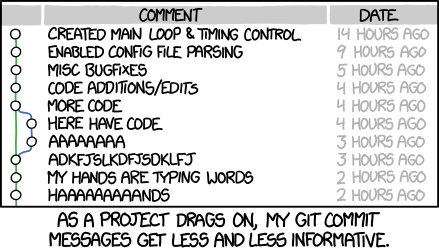
\includegraphics[width=\linewidth]{xkcd2.png}
    \caption{\url{https://xkcd.com/1296/}}
\end{subfigure}
\quad
\begin{subfigure}{.35\textwidth}
    \centering
    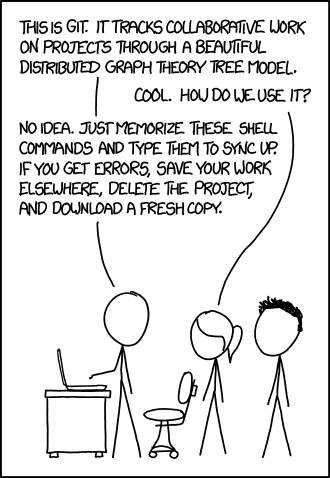
\includegraphics[width=\linewidth]{xkcd1.png}
    \caption{\url{https://xkcd.com/1597/}}
\end{subfigure}
\end{figure}

\newpage

\subsection*{Index of Git Commands} % -----------------------------------------

Execute \li{<<git help>>} for general help, or run \li{<<git help <command>>>} for instructions on a specific command.

\begin{table}[H]
\centering
\begin{tabular}{l|l}
    Command & Description \\ \hline
    \li{git status} & Display the staging area and untracked changes. \\
    \li{git pull origin master} & Pull down changes from the online repository.\\
    \li{git push origin master} & Push up changes to the online repository. \\
    \li{git add <filename(s)>} & Add a file or files to the staging area.\\
    \li{git add -u} & Add all of the modified, previously tracked files \\ & to the staging area. \\
    \li{git commit -m <<\"<message>\">>} & Save the changes in the staging area with a given \\ & message.\\
    \li{git checkout -- <filename>} & Revoke the changes made since the last commit \\ & on a file that is not in the staging area. \\
    \li{git reset -- <filename>} & Remove a file from the staging area. \\
    \li{git diff <filename>} & See the changes made on an unstaged file since \\ & the last commit. \\
    \li{git diff --cached <filename>} & See the changes made on a staged file since the \\ & last commit. \\
    \li{git log} & See the commit history (press \li{q} to exit). \\
\end{tabular}
\end{table}
